\documentclass{jsarticle}
%
\usepackage{amsmath,amssymb,bm}
\usepackage[dvipdfmx]{graphicx, color}
\usepackage{listings}
%
\setlength{\textwidth}{\fullwidth}
\setlength{\textheight}{40\baselineskip}
\addtolength{\textheight}{\topskip}
\setlength{\voffset}{-0.2in}
\setlength{\topmargin}{0pt}
\setlength{\headheight}{0pt}
\setlength{\headsep}{0pt}
%
\renewcommand{\lstlistingname}{クエリ}
\lstset{language=sql, basicstyle=\ttfamily\footnotesize, frame=single, numbers=left}
%
\title{データベース工学\\ 最終レポート}
\author{48-146427 谷川祐一}
\date{2014/08/18}
%
\begin{document}
\maketitle

\section{概要}
私は課題1のデータベースシステムの設計と性能評価に取り組んだ.以下にレポートを行う.

\section{E-R図}
データベースシステムのE-R図を図\ref{er-diagram}に示す.
営業拠点,顧客,部品,注文はそれぞれ図\ref{er-diagram}中ではbranches,customers,parts,ordersと表記している.
以下の3つの関係が存在する.
\begin{itemize}
  \item branches : orders = 1 : N
  \item customers : orders = 1 : N
  \item parts : orders = 1 : N
\end{itemize}

\begin{figure}[htbp]
  \begin{center}
    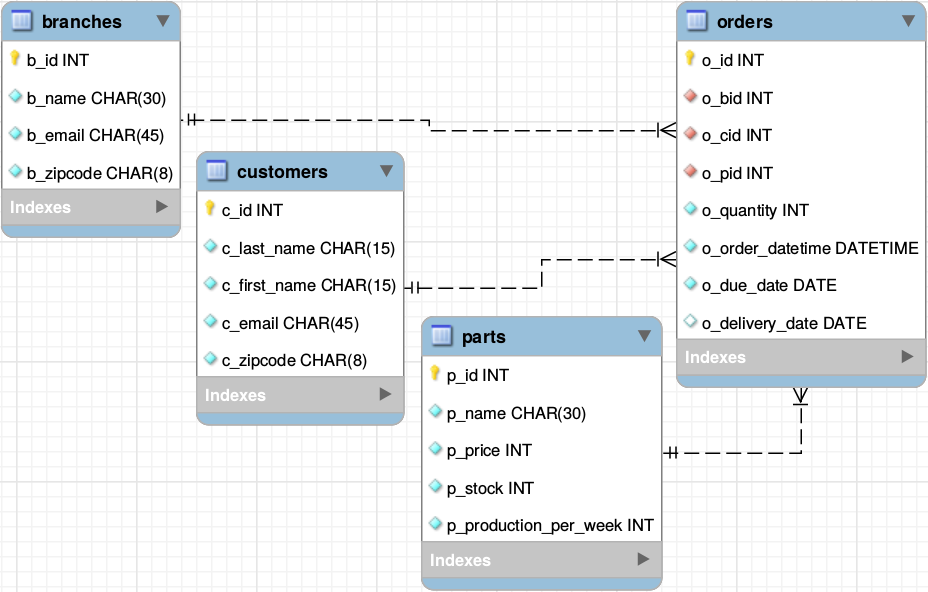
\includegraphics[width=\textwidth]{img_er_diagram.png}
  \end{center}
  \caption{E-R図}
  \label{er-diagram}
\end{figure}


\section{スキーマ設計}
E-R図を元に,branches,customers,parts,ordersからなるスキーマを設計した.以下に各実体の属性の意味を述べ,クエリ\ref{schema}にSQLで示す.

\subsection{各実体の属性の意味}

\subsubsection{branches (営業拠点)}
\begin{description}
  \item[b\_id] 重複しない拠点番号
  \item[b\_name] 営業所名
  \item[b\_email] E-mail address
  \item[b\_zipcode] 郵便番号
\end{description}

\subsubsection{customers (顧客)}
\begin{description}
  \item[c\_id] 重複しない顧客番号
  \item[c\_last\_name] 姓
  \item[c\_first\_name] 名
  \item[c\_email] E-mail address
  \item[c\_zipcode] 郵便番号
\end{description}

\subsubsection{parts (部品)}
\begin{description}
  \item[p\_id] 重複しない部品番号
  \item[p\_name] 部品名
  \item[p\_price] 価格
  \item[p\_stock] 在庫量
  \item[p\_production\_per\_week] 1週間に製造できる量
\end{description}

\subsubsection{orders (注文)}
\begin{description}
  \item[o\_id] 重複しない注文番号
  \item[o\_bid] 注文を受けた営業拠点の拠点番号
  \item[o\_cid] 注文を出した顧客の顧客番号
  \item[o\_pid] 注文された部品の部品番号
  \item[o\_quantity] 注文した個数
  \item[o\_order\_datetime] 注文日時
  \item[o\_due\_date] 見込み納期日
  \item[o\_delivery\_date] 発送日
\end{description}

\subsection{SQL}
\begin{lstlisting}[caption=スキーマのクエリ, label=schema]
CREATE TABLE `branches` (
  `b_id` INT NOT NULL,
  `b_name` CHAR(30) NOT NULL,
  `b_email` CHAR(45) NOT NULL,
  `b_zipcode` CHAR(8) NOT NULL,
  PRIMARY KEY (`b_id`));

CREATE TABLE `customers` (
  `c_id` INT NOT NULL,
  `c_last_name` CHAR(15) NOT NULL,
  `c_first_name` CHAR(15) NOT NULL,
  `c_email` CHAR(45) NOT NULL,
  `c_zipcode` CHAR(8) NOT NULL,
  PRIMARY KEY (`c_id`));

CREATE TABLE `parts` (
  `p_id` INT NOT NULL,
  `p_name` CHAR(30) NOT NULL,
  `p_price` INT NOT NULL,
  `p_stock` INT NOT NULL,
  `p_production_per_week` INT NOT NULL,
  PRIMARY KEY (`p_id`));

CREATE TABLE `orders` (
  `o_id` INT NOT NULL,
  `o_bid` INT NOT NULL,
  `o_cid` INT NOT NULL,
  `o_pid` INT NOT NULL,
  `o_quantity` INT NOT NULL,
  `o_order_datetime` DATETIME NOT NULL,
  `o_due_date` DATE NOT NULL,
  `o_delivery_date` DATE NULL,
  PRIMARY KEY (`o_id`),
  FOREIGN KEY (`o_bid`) REFERENCES `branches` (`b_id`),
  FOREIGN KEY (`o_cid`) REFERENCES `customers` (`c_id`),
  FOREIGN KEY (`o_pid`) REFERENCES `parts` (`p_id`));
\end{lstlisting}

\section{問い合わせSQLクエリ}
以下の問い合わせA,B,Cを行うSQLクエリをそれぞれ示す.

\subsection{A. 1個3,000円以上の部品を1度でも買ったことのある顧客の姓名を出力}
クエリ\ref{q1a}と\ref{q1b}の2通り考えられる.

\begin{lstlisting}[caption=問い合わせAのクエリ(1), label=q1a]
SELECT DISTINCT
    c_last_name, c_first_name
FROM
    customers, parts, orders
WHERE
    c_id = o_cid
	AND p_id = o_pid
    AND p_price >= 3000;
\end{lstlisting}

\begin{lstlisting}[caption=問い合わせAのクエリ(2), label=q1b]
SELECT
    c_last_name, c_first_name
FROM
    customers
WHERE
    EXISTS (
        SELECT
            *
        FROM
            orders, parts
        WHERE
            c_id = o_cid
            AND p_id = o_pid
            AND p_price >= 3000);
\end{lstlisting}

\subsection{B. 自分の住む同じ都道府県にある営業拠点からだけ購入している顧客の姓名を出力}
\begin{lstlisting}[caption=問い合わせBのクエリ, label=q2]
SELECT
    c_last_name, c_first_name
FROM
    customers
WHERE
    SUBSTRING(c_zipcode, 1, 2) = ALL (
        SELECT
            SUBSTRING(b_zipcode, 1, 2)
        FROM
            branches,
            orders
        WHERE
            c_id = o_cid
            AND b_id = o_bid);
\end{lstlisting}

\subsection{C. 全ての注文についての平均の納品日数を出力}
\begin{lstlisting}[caption=問い合わせCのクエリ, label=q3]
SELECT
    AVG(DATEDIFF(o_delivery_date, o_order_datetime))
FROM
    orders;
\end{lstlisting}

\section{SQLクエリの性能測定}
前述のSQLクエリについて,RDSを利用して性能測定を行った.
測定環境,利用したデータセット,測定方法,測定結果を順に述べる.

\subsection{測定環境}
\begin{description}
  \item[DB Engine] mysql
  \item[DB Engine Version] 5.6.17
  \item[DB Instance Class] db.t1.micro, 1 vCPU, 0.613 GiB RAM
  \item[Multi-AZ Deployment] No
  \item[Allocated Storage] 5 GB
  \item[Use Provisioned IOPS] No
  \item[innodb\_buffer\_pool\_size] 295 MiB
\end{description}

\subsection{利用したデータセット}
TPC-Hベンチマーク\cite{tpch}のスキーマを参考にしてテストデータを生成するプログラムを作成し,それを利用してテストデータを生成した.
以下に生成アルゴリズムと生成したデータサイズについて述べる.

\subsubsection{生成アルゴリズム}
以下に各属性の生成アルゴリズムを述べる.
問い合わせAとBにおいて0や1のような極端なセレクティビティを避けてある程度のセレクティビティを確保するための生成規則については,\ref{selectivity-for-a}と\ref{selectivity-for-b}で後述する.

アルゴリズム中では名前やE-mail addressなどの値は現実には意味をなさないものとなっているが,テストデータとしては妥当だと考える.

\subsubsection*{branches}
\begin{description}
  \item[b\_id INT] 1から始まる一意な連番の整数.
  \item[b\_name CHAR(30)] "Branch$\sharp$000000001"のように,"Branch$\sharp$"の後にb\_idを9桁の右詰めゼロ詰めの固定長の文字列にして結合した文字列.
  \item[b\_email CHAR(45)] "Branch$\sharp$000000001@example.com"のように,b\_nameの後に"@example.com"を結合した文字列.
  \item[b\_zipcode CHAR(8)] "ddd-dddd"なる文字列.dは0から9のランダムな数値とする.ただし後述する\ref{selectivity-for-b}の生成規則を適用する.
\end{description}

\subsubsection*{customers}
\begin{description}
  \item[c\_id INT] 1から始まる一意な連番の整数.
  \item[c\_last\_name CHAR(15)] "Customer"なる文字列.
  \item[c\_first\_name CHAR(15)] "$\sharp$000000001"のように,"$\sharp$"の後にc\_idを9桁の右詰めゼロ詰めの固定長の文字列にして結合した文字列.
  \item[c\_email CHAR(45)] "Customer$\sharp$000000001@example.com"のように,c\_last\_name, c\_first\_name, "@example.com"を結合した文字列.
  \item[c\_zipcode CHAR(8)] "ddd-dddd"なる文字列.dは0から9のランダムな数値とする.ただし後述する\ref{selectivity-for-b}の生成規則を適用する.
\end{description}

\subsubsection*{parts}
\begin{description}
  \item[p\_id INT] 1から始まる一意な連番の整数.
  \item[p\_name CHAR(30)] "Part$\sharp$000000001"のように,"Part$\sharp$"の後にp\_idを9桁の右詰めゼロ詰めの固定長の文字列にして結合した文字列.
  \item[p\_price INT] 100から3050までのランダムな整数.範囲の決め方は後述する\ref{selectivity-for-a}による.
  \item[p\_stock INT] 100から1000までのランダムな整数.性能測定するクエリのセレクティビティには関係ないので,範囲は適当に決めた.
  \item[p\_production\_per\_week INT] 100から1000までのランダムな整数.同上.
\end{description}

\subsubsection*{orders}
\begin{description}
  \item[o\_id INT] 1から始まる一意な連番の整数
  \item[o\_bid INT] 1からb\_idの最大値までのランダムな整数.ただし後述する\ref{selectivity-for-b}の生成規則を適用する.
  \item[o\_cid INT] 1からc\_idの最大値までのランダムな整数.ただし後述する\ref{selectivity-for-b}の生成規則を適用する.
  \item[o\_pid INT] 1からp\_idの最大値までのランダムな整数.
  \item[o\_quantity INT] 1から50までのランダムな整数.
  \item[o\_order\_datetime DATETIME] 2013年0時0分0秒から2013年12月16日23時59分59秒までのランダムな日時.
  \item[o\_due\_date DATE] 納期までの日数dueを1から10のランダムな整数とし,dueをo\_order\_datetimeの日付に加えた日付.
  \item[o\_delivery\_date DATE] dueに0.5から1.5までのランダムな実数(プログラム上はdouble)を掛けたものをo\_order\_datetimeの日付に加えた日付.
    o\_delivery\_dateが最大でも2013年12月31日に収まるようにこれら3つの日時と日付を設定した.また問い合わせCの平均納品日数は約5.5日となる.
\end{description}

\subsubsection{データサイズ}
表\ref{data-size}に示すサイズのデータを作成した.
容量の概算には表\ref{sizeof-type}に示すデータ型のバイト数\cite{mysql-data-type-size}を用いた.
\begin{table}[htb]
  \begin{center}
    \caption{データサイズ}
    \label{data-size}
    \begin{tabular}{|c|c|c|}\hline
      テーブル & 行数 & 容量(概算) [MB] \\ \hline
      branches & 10,000 & 0.82 \\
      customers & 150,000 & 13.05 \\
      parts & 200,000 & 9.2 \\
      orders & 3,000,000 & 93 \\ \hline
      合計 & - & 116.07 \\ \hline
    \end{tabular}
  \end{center}
\end{table}

\begin{table}[htb]
  \begin{center}
    \caption{データ型のバイト数}
    \label{sizeof-type}
    \begin{tabular}{|c|c|c|c|}\hline
      INT & CHAR(X) & DATETIME & DATE \\ \hline
      4 & X & 5 & 3 \\ \hline
    \end{tabular}
  \end{center}
\end{table}

\subsubsection{問い合わせAのセレクティビティのための生成規則}
\label{selectivity-for-a}
問い合わせAのcustomersに対するセレクティビティの概算は,3,000円以上の部品の割合を$ p $,顧客1人当たり平均注文回数を$ n $とすると,
\[
  1 - (1 - p)^{n}
\]
となる.
生成したデータサイズから$ n = 20 $であり,部品の価格のランダムな100から3,050の整数とすると$ p = 0.017 $となり,セレクティビティは$ 0.29 $となる.

\subsubsection{問い合わせBのセレクティビティのための生成規則}
\label{selectivity-for-b}
問い合わせBのcustomersに対するセレクティビティの概算は,顧客が同じ都道府県の営業拠点から注文する確率を$ q $,顧客1人当たり平均購入回数を$ n $とすると,
\[ 
  q ^ {n}
\]
となる.
生成したデータサイズから$ n = 20 $であり,仮に$ q = 0.9 $とすると,セレクティビティは$ 0.1 $となる.

$ q = 0.9 $を実現するために,以下のような生成規則を導入する.
\begin{description}
  \item[b\_zipcodeとc\_zipcode] それぞれ先頭2文字を,b\_idの下2桁,c\_idの下2桁とする.すなわち拠点番号と顧客番号の下2桁で都道府県を表すようにする.
  \item[o\_bidとo\_cid] $ 0.9 $の確率で下2桁を同じ番号として生成する.
\end{description}

\subsection{測定方法}
問い合わせAのクエリ\ref{q1a}と\ref{q1b},問い合わせBのクエリ\ref{q2},問い合わせCのクエリ\ref{q3}について,それぞれ外部キーのインデックスの有無の2通りについて5回づつ実行して,実行時間の平均と標準偏差を求めた.またクエリ\ref{q1a}については,外部キーのインデックスに加えてp\_priceにセカンダリインデックスを作成した場合についても測定を行った.

なおキャッシュの効果を回避するために以下の方法で測定を行った.
まず,テストデータとは別に800MBほどのダミーデータをデータベースに作成した.
各問い合わせクエリの実行前には,ダミーデータのテーブルをクエリ\ref{qdummy}を用いてフルテーブルスキャンを行い.その後RDSのDB instanceを再起動させた.

RDSではDBMSより低レイヤのキャッシュを明示的にクリアする方法は見当たらなかったので,0.613 GiBのメモリサイズを超えるダミーデータを読み込むことで実質的にキャッシュからテストデータを追い出したとみなした.
DBMSのキャッシュについては,DB instanceを再起動することでクリアしたとみなした.

\begin{lstlisting}[caption=ダミーデータをフルスキャンする, label=qdummy]
SELECT
    count(*)
FROM
    dummy;
\end{lstlisting}

\subsection{測定結果}
実行時間の平均と標準偏差を表\ref{result}に示す.

外部キーインデックスがない場合のクエリ\ref{q1b}とクエリ\ref{q2}はそれぞれ2〜3時間ほど実行してみたものの終わらなかったので,今回は測定不能とみなした.

\begin{table}[htb]
  \begin{center}
    \caption{問い合わせクエリの実行時間の平均と標準偏差}
    \label{result}
    \begin{tabular}{|c|c|c|c|c|}\hline
      問い合わせ & クエリ & インデックス & 平均[秒] & 標準偏差[秒] \\ \hline
      A & \ref{q1a} & 外部キー & 22.92 & 0.15 \\
        & \ref{q1a} & 外部キー + p\_price & 21.33 & 0.22 \\
        & \ref{q1a} & - & 18.38 & 0.16 \\
        & \ref{q1b} & 外部キー & 31.16 & 0.65 \\
        & \ref{q1b} & - & 測定不能 & 測定不能 \\ \hline
      B & \ref{q2} & 外部キー & 25.29 & 0.86 \\
        & \ref{q2} & - & 測定不能 & 測定不能 \\ \hline
      C & \ref{q3} & 外部キー & 13.44 & 0.09 \\
        & \ref{q3} & - & 13.57 & 0.3 \\ \hline
    \end{tabular}
  \end{center}
\end{table}

\subsection{考察}
問い合わせAのクエリ\ref{q1a}で外部キーインデックスがある場合の実行計画は,partsテーブルにアクセスした後に外部キーを用いてordersテーブルをジョインし,その後プライマリキーを用いてcustomersテーブルをジョインするというものだった.
p\_priceのセカンダリインデックスの有無で少しだけしか実行時間が変わらなかったのは,p\_priceの値をインデックスから読むか実テーブルから読むかにかかる時間よりも,他のテーブルとのジョインするためにディスクに対するランダムアクセスをする時間が支配的だからだと考えられる.
今回は実験できなかったが,3,000円以上の部品の割合が今よりも極端に0に近い場合だと,p\_priceのセカンダリインデックスは有効に働くと考えられる.

また外部キーインデックスがない場合の\ref{q1a}の実行計画は,ordersテーブルにアクセスした後にcustomersテーブルとpartsテーブルをそれらのプライマリキーを用いてジョインするというものだった.
このとき実行時間が外部キーありの場合よりも短くなったのは,MySQLのデータ構造上セカンダリインデックスを使う場合,セカンダリキーのインデックスを引いて取得したプライマリキーの値で実データを取得するということを行っているので,セカンダリインデックスを引くという二度手間をせず直接プライマリキーでデータにアクセスできたためだと考えられる.
MySQLのオプティマイザが本当に最適な実行計画を出せるかいうと,そうではないということが窺い知れる.

問い合わせAのクエリ\ref{q1b}と問い合わせBのクエリ\ref{q2}の実行計画は,customersテーブルにアクセスした後,キーを用いずに相関サブクエリが実行されていた.
サブクエリ中では,ordersテーブルにアクセスした後,プライマリキーを用いてそれぞれpartsとbranchesテーブルをジョインしていた.
キーを用いない相関サブクエリなのでネスティッドループが用いられていると仮定すると,その時間計算量はテーブルの行数に換算して
\[ 
  \rm (外部クエリの行数) \cdot (内部クエリの行数) = |customers| \cdot |orders| = 15,000 \cdot 3,000,000 = 4.5 \cdot 10^{11}
\]
と大きいことがわかる.

問い合わせCのクエリ\ref{q3}についてはordersテーブルをフルテーブルスキャンするので,外部キーインデックスの有無で実行時間は変化しない.

\begin{thebibliography}{9}
  \bibitem{tpch} TPC $\rm Benchmark^{TM}$ H Standard Specification Revision 2.17.0 (Apr. 2014).
  \bibitem{mysql-data-type-size} MySQL :: MySQL 5.6 Reference Manual :: 11.7 Data Type Storage Requirements. http://dev.mysql.com/doc/refman/5.6/en/storage-requirements.html
\end{thebibliography}

\end{document}